\chapter{Introduction}
\label{sec:intro}

\section{Thesis Statement}

This dissertation explores two problems in balancing software performance and system energy consumption in computing systems: (1) meeting application performance goals while minimizing energy consumption, and (2) running applications as energy-efficiently as possible.
We address the first problem using control theory to meet performance goals by tuning system knobs such as DVFS frequencies, core allocations, and hardware power caps.
We treat the second as a classification problem, using machine learning classifiers, driven by low-level hardware counter metrics, to predict the most energy-efficient system knob settings at runtime.


\section{Problem Description}
\label{sec:intro-description}

Performance and energy consumption are conflicting goals in computing systems and must be appropriately balanced to satisfy user requirements.
As power and energy become first-class concerns in systems ranging from low-power embedded platforms to large-scale High Performance Computing (HPC) environments, there is an increasing need for software to manage hardware resource allocations to achieve a desirable balance in performance and power/energy consumption.
Fortunately, modern systems expose knobs to support trading performance and power.

For example, Dynamic Voltage and Frequency Scaling (DVFS) trades processor clock rate and power consumption for changes in throughput, and is ubiquitous in modern systems.
Dynamic power $P$ is proportional to the effective capacitance $C$ of a processor, the applied voltage $V$, and the clock frequency $f$ \cite{Hennessy:2003:CAQ:861856}:
\begin{equation}
P \propto \frac{1}{2}CV^2f
\label{eqn:bg-power}
\end{equation}
Higher clock frequencies typically result in higher performance, \eg for compute-bound applications.
However, voltage and frequency are correlated, meaning their values in \eqnref{bg-power} cannot be adjusted independently \cite{LeSueur2010}.
% Thermal design constraints limit the power consumption that a computing system can sustain, in turn limiting both the maximum and average performance that can be achieved.
Higher clock frequencies require higher voltage to maintain stable circuit operation; conversely, lower frequencies can maintain operation at lower voltages.
Reducing the voltage and frequency can offer significant power savings due to this non-linear relationship.
Newer technologies allow specifying power caps for hardware resources and letting the components optimize their own behavior subject to the power constraint, \eg Intel Running Average Power Limit (RAPL) tunes DVFS much faster than software \cite{RAPL}.
Another common knob setting is the allocation of compute cores on multicore systems, allowing unallocated cores to enter low-power sleep states, or even shut down altogether to save power/energy.

If we consider each allowable combination of knob values to be a system \emph{setting} or \emph{configuration}, we can explore the impact of different knob combinations on performance and power consumption.
Therefore, to understand the behavior of a particular application on a system, we can perform a characterization by testing the application in each system configuration and recording the behavior.
The result is a \emph{tradeoff space}, where each system configuration produces unique application performance and system power values.
Often only a subset of the available configurations are actually desirable---it is straightforward to derive the Pareto-optimal configurations, or even those that lie on the (upper or lower) convex hull of the tradeoff space.

A significant amount of software is subject to performance requirements.
Power or energy can then be optimized under the performance constraint to increase battery life or reduce power costs.
Until recently, heuristic approaches were often sufficient to meet performance goals while achieving near-minimal energy consumption.
However, heuristic approaches to balancing performance and power/energy rely on assumptions about the performance/power tradeoff space of an application and system that we have found are not portable between applications and modern systems.
For example, the classic \emph{race-to-idle} heuristic can achieve low energy consumption on one system, but high energy consumption on another compared with a \emph{pace-to-idle} or \emph{never-idle} approach \cite{Imes2014}.
While performance/power tradeoff spaces were mostly linear on older systems, advances in technology are making them more convex on modern systems.
An important observation by Kim \etal is, ``Unless the function of a given machine is a straight line originating from the idle state, (0, $P_{idle}$), an idling heuristic is never optimal for all instances'' \cite{kim-cpsna2015}.
In short, the more convex the tradeoff space, the further from optimal any idling approach is.

A more optimal tradeoff in balancing performance and power is to maximize \emph{energy efficiency}, \ie the amount of work completed per unit of energy consumed (analogous to maximizing the ratio of performance to power).
Sometimes it is desirable simply to reduce the energy cost of a computation at the expense of slower execution.
In the High Performance Computing (HPC) domain, maximizing energy efficiency can maximize the throughput of power-constrained, hardware over-provisioned clusters \cite{PatkiRMAP}.
As with meeting performance goals, a similar problem with heuristics arises---the optimal approach varies between applications and systems.


\begin{figure}[t]
  \begin{centering}
  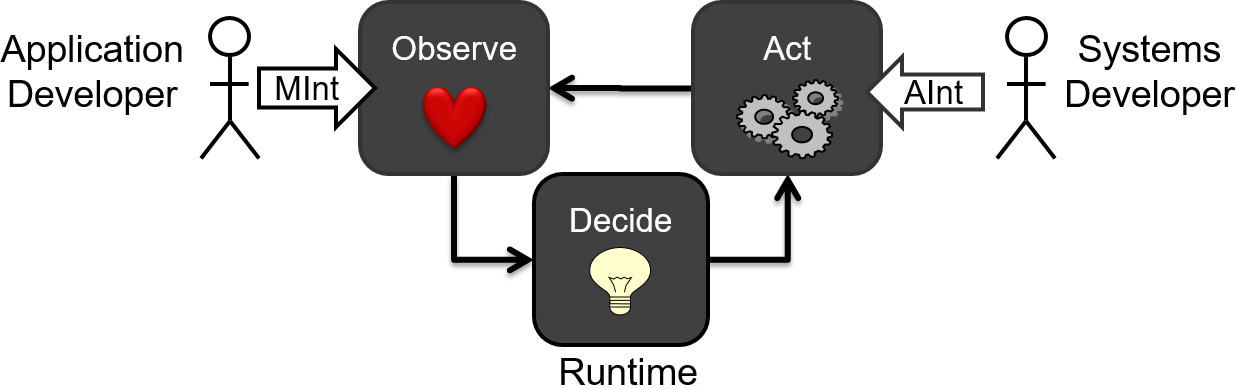
\includegraphics[width=0.6\textwidth]{figs/SEEC.png}
  \caption{A self-aware computing (SEEC) runtime model -- observe, decide, and act.}
  \label{fig:seec}
  \end{centering}
\end{figure}

The lack of both portability and optimality of heuristics demand that we develop more general approaches to addressing the problems in balancing performance and power/energy.
In his PhD dissertation, Hoffmann proposes a ``self-aware'' computing model (SEEC) that uses a closed-loop feedback design to \emph{observe}, \emph{decide}, and \emph{act} \cite{HoffmannPhD}.
\figref{seec} demonstrates this concept.
The SEEC model is more portable than many heuristics because it includes an observation step that measures behavior at runtime rather than relying strictly on assumptions made offline.
We build on this high-level model and use feedback systems that measure application and system behavior during runtime to make informed changes to resource allocations as new information becomes available.
Furthermore, our general feedback system designs do not depend on extremely accurate or complete models.
Instead, they rely on runtime measurements to fine-tune their decisions.


\section{Contributions}

This dissertation addresses two common goals in managing software performance and system energy consumption.
The first is the constrained optimization problem of meeting an application performance goal while minimizing energy consumption.
Software performance constraints are common in applications that run on platforms ranging from embedded to server-class.
% , \eg cloud-based software that must meet quality-of-service guarantees.
The second addresses the problem of running software as energy-efficiently as possible, \ie maximizing the ratio of work completed to energy consumed.
% Maximizing energy efficiency is particularly beneficial in HPC, where systems should be kept busy while reducing the cost of scientific insight.
We address these two problems with three distinct projects:
\begin{itemize}
\item POET, the \textbf{P}erformance with \textbf{O}ptimal \textbf{E}nergy \textbf{T}oolkit: A portable, control-theoretic framework for meeting soft application performance goals while optimizing energy consumption, which we demonstrate by tuning DVFS settings and core allocations.
\item CoPPer, \textbf{Co}ntrol \textbf{P}erformance with \textbf{P}ow\textbf{er}: A model-free, control-theoretic approach for meeting soft application performance constraints by tuning processor power caps and allowing the hardware to optimize energy consumption.
\item CEES, \textbf{C}lassification of \textbf{E}nergy-\textbf{e}fficient \textbf{S}ettings: A machine learning classification framework for predicting energy-efficient system settings based on low-level hardware performance counter metrics, which we demonstrate by tuning DVFS, socket allocations, and the use of HyperThreads.
\end{itemize}
\appref{tools} describes portable tools created to support these projects that we believe are useful to other researchers and developers.
\appref{urls} provides open-source release information for POET, CoPPer, and supporting tools.


\subsection{POET}

POET addresses the problem of meeting soft real-time application performance goals while minimizing energy consumption.
A significant amount of software is subject to performance constraints, from applications running on low-power embedded platforms to those in high-performance, high-power environments like on servers in datacenters.
Optimizing energy consumption increases the usable runtime of battery-powered systems like tablets, smartphones, and smaller devices we now classify as Internet of Things; for always-on devices, it reduces the runtime energy costs.

Kim \etal prove that an optimal solution to this constrained optimization problem requires, at most, two system configurations from the convex hull of the tradeoff space \cite{kim-cpsna2015}.
POET uses control theory to meet the performance goal and linear optimization to select the optimal pair of system configurations that satisfy the performance constraint.
While POET was originally designed for embedded systems \cite{POET}, we later evaluated it on a server-class system \cite{POETMCSoC}.

POET's evaluation uses DVFS and core allocation as the system knobs to control performance and energy consumption.
While significant prior work has used these knobs, their solutions tend to be restricted to particular applications and systems, limiting their portability.
In contrast, POET's design is independent of any particular application or platform and their performance/power tradeoff spaces.

We find that POET achieves:
\begin{itemize}
\item \textbf{Ease of Use}: Integrating POET with applications only requires a few additional lines of code.
\item \textbf{Predictable Performance}: POET meets a range of performance targets, minimizing the error between the goal and the achieved performance.
\item \textbf{Energy Savings}: Using an offline oracle, we verify that POET achieves near-optimal energy consumption (\eg 1.3\% over optimal on an Intel-powered tablet, 2.9\% on an ARM big.LITTLE system), which includes POET's runtime overhead.
\item \textbf{Adaptability}: POET adapts to phases in application and input behavior, achieving increased energy savings during periods of low computational demand.
Additionally, POET adapts to noise in the system introduced by co-scheduled applications to ensure that performance goals are still met when feasible, and makes a best effort otherwise.
\end{itemize}


\subsection{CoPPer}

CoPPer also addresses the problem of optimizing energy consumption under a soft performance constraint, but does so by tuning hardware power caps.
Recent trends suggest that software control of DVFS is being deprecated, making all prior software approaches that depend on DVFS obsolete.
Linux kernel developers have acknowledged this trend \cite{lwn602479}.
In fact, the Linux kernel documentation notes, ``the idea that frequency can be set to a single frequency is fictional for Intel Core processors. Even if the scaling driver selects a single P-State, the actual frequency the processor will run at is selected by the processor itself'' \cite{KernelPstate}.

However, hardware is not aware of application-level performance requirements, so a software component is still needed to ensure that performance constraints are respected.
Fortunately, emerging interfaces let software set \emph{power caps} on hardware, with hardware free to determine what DVFS frequencies should be used and when, so long as the average power over some time window is respected.
For example, Intel's Running Average Power Limit (RAPL) allows software to set power limits on hardware \cite{RAPL}.
This poses a new challenge.
Meeting performance constraints with DVFS is easy: simple linear models map changes in processor clock frequency to changes in application performance.
Meeting performance requirements with power capping is harder: power and speedup have a non-linear relationship (\eqnref{bg-power}) and most applications exhibit diminishing performance returns with increasing clock frequency (and thus power), \ie are not entirely compute-bound.

CoPPer proposes to leverage hardware power capping to control performance, leaving the energy optimization to the hardware.
Its evaluation uses Intel RAPL, which manages DVFS in hardware at finer-grained intervals than software can, while strictly respecting the imposed power limit.
CoPPer makes the following contributions:
\begin{itemize}
\item Demonstrates the need for a DVFS alternative that allows software to manage performance/power tradeoffs.
\item Proposes software-defined power capping as a replacement for software-managed DVFS.
\item Presents CoPPer, a feedback controller that meets performance goals by manipulating hardware power caps, handles non-linearity in power cap/performance tradeoffs, and introduces adaptive \emph{gain limits} to further reduce power when it does not increase performance.
\item Evaluates CoPPer using Intel RAPL on a dual-socket, 32-core server.
We find that CoPPer achieves performance guarantees similar to software DVFS control, but with better energy efficiency.
Specifically, CoPPer improves energy efficiency by 6\% on average with a 12\% improvement for memory-bound applications.
At the highest performance targets, CoPPer's gain limit saves even more energy: 8\% on average and 18\% for memory-bound applications.
\end{itemize}


\subsection{CEES}
\label{sec:intro-ee}

In other scenarios, it is desirable to maximize energy efficiency, \ie complete a fixed-size computation using the least energy possible without a performance constraint.
It is becoming well-established that the \emph{race-to-idle} heuristic is not energy-efficient.
% Our discussion of \emph{race-to-idle} in the context of performance constraints earlier is irrelevant, since if that heuristic cannot meet a constraint, no other approach can.
It may then seem reasonable to simply run in the lowest-power system configuration, but this approach fails to account for elapsed time, so energy consumption may still exceed optimal even when consuming low power.
Identifying the most energy-efficient system setting is challenging since the optimal setting varies depending on varying application resource demands.

We address this problem in the High Performance Computing (HPC) domain.
It has historically been desirable in HPC to run software as fast as possible.
The motivation behind this approach is either to: (1) get an answer to a scientific question as fast as possible, or (2) for the HPC cluster to complete as much work as possible, \ie maximize the cluster throughput.
The goal of completing an application as fast as possible leaves little room for power/energy optimization, although some work has been done in this area (see \secref{related}).
Until recently, maximizing application performance also solved the latter problem.
Now we are moving toward the era of exascale systems with strict power budgets \cite{Exascale20MW}.
Hardware over-provisioning, which allows more systems to operate in a cluster than can actually be supported if each were consuming their maximum power budget, has been proposed as an approach to improve cluster throughput \cite{PatkiRMAP}.
It works because systems do not usually require their maximum allowable power budget.
In these new hardware over-provisioned, power-constrained clusters, maximizing energy efficiency instead of application performance will both decrease the cost of per-application scientific insight and maximize the throughput of the cluster.

Our solution is to treat this challenge as a classification problem, using samples from low-level hardware performance counters to drive machine learning algorithms that predict the most energy-efficient configuration to use.
This approach does not require the software to provide its own instrumentation, nor does the classifier need to know anything about the application in advance.
Using classification instead of estimation reduces the computational overhead of the software solution, at the cost of less insight into the resource predictor's decision.
We tune DVFS, socket allocation, and the use of HyperThreads.

This work makes the following contributions:
\begin{itemize}
\item Proposes optimizing \emph{energy efficiency} instead of \emph{runtime} to decrease the cost of scientific computation.
\item Establishes the problem complexity---of 15 different machine learning classification techniques evaluated, only some are suitable for optimizing energy efficiency.
\item Demonstrates that sufficiently powerful classifiers can dramatically reduce energy consumption by accurately predicting energy-efficient system settings at runtime.
\item Extrapolates from empirical results to posit that optimizing energy efficiency can improve the throughput of hardware over-provisioned, power-constrained systems by up to 24\%.
\end{itemize}
